%!TEX root = ../template.tex
%%%%%%%%%%%%%%%%%%%%%%%%%%%%%%%%%%%%%%%%%%%%%%%%%%%%%%%%%%%%%%%%%%%%
%% chapter2.tex
%% NOVA thesis document file
%%
%% Chapter with the template manual
%%%%%%%%%%%%%%%%%%%%%%%%%%%%%%%%%%%%%%%%%%%%%%%%%%%%%%%%%%%%%%%%%%%%

\typeout{NT FILE chapter2.tex}%

\chapter{Literature Review}
\label{cha:literaturereview}

\textit{This section provides an overview of the relevant research related to the topic of the project.
First, it begins by highlighting the importance of understanding the \gls{MoA} in \gls{DD}, followed by a description of two fundamental components for \gls{MoA} elucidation: transcriptomic data and biological networks.
Then, the computational methods used to apply various scoring algorithms (topology-, similarity-, and enrichment-based algorithms) are summarized, laying the groundwork for a systematic evaluation of tools designed to infer compound \gls{MoA}.
Finally, the section outlines best practices for conducting a benchmarking study.}

\section{Drug discovery: the importance of the compound's mechanism of action} % (fold)
\label{sec:drugdiscoverytheimportanceofthecompoundsmechanismofaction}

Developing new drugs is an extraordinarily complex process.
The high prevalence of complex diseases, which collectively account for 70\% of all the deaths in Europe and affect around 25\% of the population, is one of the challenges faced by this industry~\cite{RN43}.
In addition, statistics show that \textit{de novo} \gls{DD} has become an extensive and costly process, taking on average 13 years and 2\$ billion to develop a new drug, with most of clinical trials lasting 95 months and non-clinical development 31 months~\cite{RN55,RN56,RN47}.
These challenges have led to fewer drug approvals by regulatory bodies, resulting in a significant gap between therapeutic demand and available treatments. Hence, as the current treatments become less effective, there is a strong interest in finding alternatives to optimize critical steps in the drug development pipeline and developing more advanced therapeutic methods~\cite{RN44}.
Efforts to address these challenges are evident in the growing number of studies, both in industry and academia.

\gls{DR} emerged as a promising cost-effective strategy to tackle the constraints faced by traditional \gls{DD} by reducing the initial cost to 1/3 and the duration to 3-9 years, and it continues to gain increasing attention, as nearly 30\% of the drugs approved by the \gls{FDA} are identified using this approach~\cite{RN54,RN64}. 
The fundamental goal of \gls{DR} is to broaden the indication of known, safe, and previously approved drugs. 
From multiple points of view, this is a particularly interesting approach. 
It allows to investigate therapeutic agents that have been put on hold because of failed clinical trials~\cite{RN62}, and also it enables to identify treatment for conditions with unmeet clinical needs. 
This is the case of rare diseases, which are not providing sufficient returns to pharmaceutical companies to justify a conventional \gls{DD} pipeline. 
Many studies have demonstrated the success of establishing new drug-disease relationships~\cite{RN48}. 
A well-known example is Sildenafil; initially identified in the 1980s as a candidate to treat angina pectoris, it was approved by the \gls{FDA} in 1998 to treat erectile dysfunction and later in 2005 to treat pulmonary arterial hypertension~\cite{RN54, RN64, RN94}. 
Another classic example is Thalidomide, originally used for sedation and morning sickness, and afterward repurposed for multiple myeloma, leprosy~\cite{RN54, RN64}, and to minimize the hippocampal neuronal loss~\cite{RN50}. Moreover, the low success rate (5\%) for phase I clinical studies of cancer treatments led to increased attention in \gls{DR} for oncology, resulting in several promising findings~\cite{RN64, RN63}. 
Noteworthy cases include the schizophrenia drug Spiperone, which has been studied for its ability to induce apoptosis in \gls{CRC} cells~\cite{RN51}, and Raloxifene, indicated for osteoporosis, which proved to be effective in reducing breast cancer risk in postmenopausal women~\cite{RN64, RN61}.

Understanding how cellular signaling (Figure~\ref{fig:fig2.1.cellularsignalingcascade}) is modulated upon a stimulus is essential for identifying potential drug targets and finding new indications for an existing drug. 
When a drug enters a biological system, it typically interacts directly or indirectly with cellular targets, regulating the activity of signaling networks and pathways. 
This is commonly referred as the \gls{MoA}~\cite{RN52, RN53}. These interactions are relevant across the whole \gls{DD} process, from initial investigation to clinical trials. A deep understanding of a drug's \gls{MoA} allows to uncover drug-exposure biomarkers, anticipate early adverse effects, and even synergistic effects resulting from drug combinations. 
Nevertheless, FDA approval can be obtained without knowing the drug's \gls{MoA} if the drug exhibits sufficient safety and efficacy~\cite{RN38, RN68}. 
Yet, not knowing the mechanisms of the compounds can be extremely disadvantageous. This is demonstrated by the case of Dimebon. 
Originally developed as an antihistamine drug, it later entered clinical trials (with the \gls{MoA} still unknown) for the treatment of Alzheimer's disease, failing to show meaningful clinical efficacy in phase 3 studies. 
Later, it was clarified that it was the activity on the histamine and serotonin receptors that caused the initial observed cognitive efficacy, instead of the stabilization of mitochondria (as first hypothesized)~\cite{RN38, RN69}.

\begin{figure}[htbp]
    \centering
    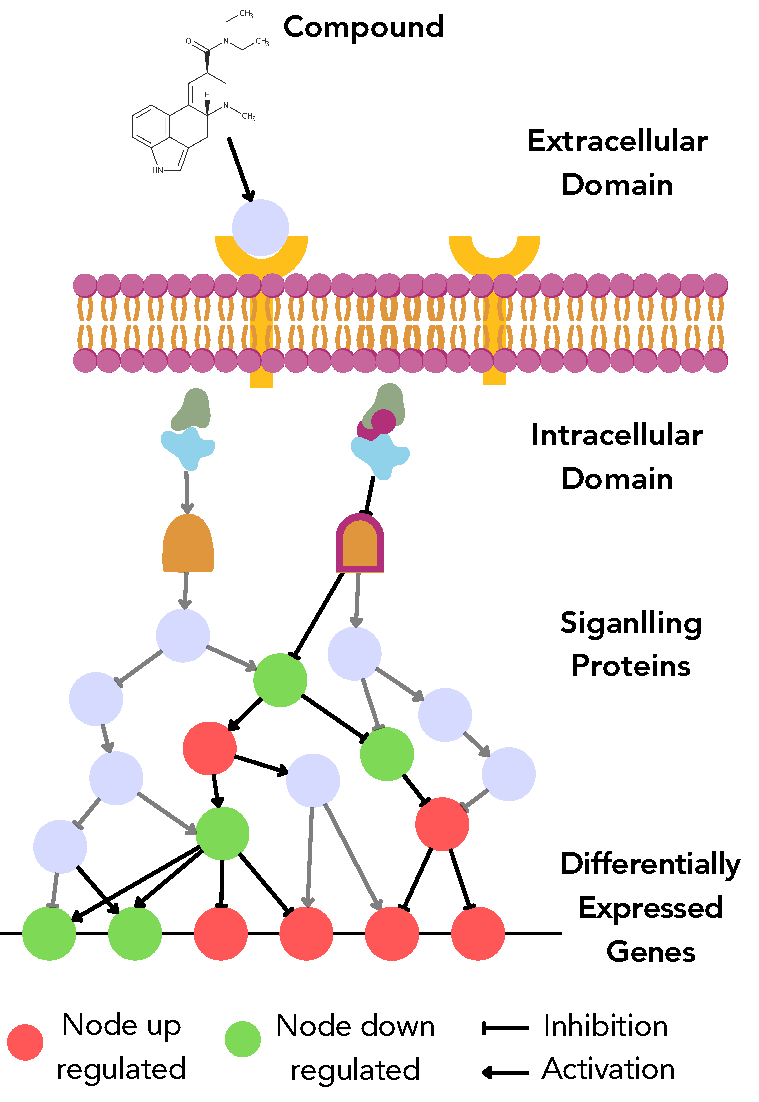
\includegraphics[height=4in]{fig2.1.cellularsignalingcascade}
    \caption[Schematic representation of a compound-induced cellular signaling cascade.]{Schematic representation of a compound-induced cellular signaling cascade, where binding of the perturbing compound to its extracellular receptor domain triggers downstream intracellular signal transduction events through various signaling proteins, ultimately altering gene expression levels in the nucleus. The red nodes represent upregulated genes, the green nodes represent downregulated genes, arrows denote activation events, and T-bar edges indicate inhibitory interactions.}
    \label{fig:fig2.1.cellularsignalingcascade}
\end{figure}

Although we refer to the target(s) of a compound as direct, this is often not the case. 
From a chronological point of view, there are a series of interactions that result in modulation of biological processes, and what is detected at a given moment does not always linearly reflect what happened previously. 
Indeed, the basic definition of \gls{MoA} is just the tip of the iceberg, given the chain of biochemical reactions forming part of the cell signaling cascade. 
This process is characterized by the signaling pathways leading to a certain cellular response. These pathways can also interact with each other through crosstalk~\cite{RN94}, forming a complex network of interconnected and distinct nodes. 
The impact of a certain compound in the complex cell signaling cascade can be defined and observed on a system level by high throughput approaches such as Genomics, \gls{Transcriptomics}, Proteomics, Metabolomics, and even Phenomics. 
Each of them provides a different perspective on the compound's activity. 
Despite these technological progresses, experimental identification of targets, signaling proteins, and biological pathways (\gls{MoA}) modulated by an uncharacterized compound can be extremely difficult. 
To facilitate this process \gls{HTS} \textit{in silico} methods have become an attractive option, given the affordability, speed and the amount of data provided. 
These methods act as a screening process, helping to identify and produce mechanistic hypotheses for further experimental validation~\cite{RN38}. 
Many accessible computational resources integrate omics data with prior knowledge graphs, such as \gls{GRN}, to enhance and pinpoint the drug's potential cellular targets. 
However, choosing the most suitable data and computational tool for each situation is not always simple, requiring precise identification of the scientific question that needs to be addressed. 
By doing this, researchers can choose the most appropriate data type and bioinformatics tools to efficiently study a compound's \gls{MoA}.

\section{Transcriptomic data}
\label{sec:Transcriptomicdata}

Transcriptomic data provides a comprehensive view of gene expression changes in response to a compound. 
Following the compound's perturbation, these data will reflect the differential \gls{mRNA} expression, by capturing modulated signaling and \gls{TF} activity changes triggered by the perturbagen.
For this reason, after a cellular disturbance, changes in gene expression levels give rise to a perturbated gene expression signature~\cite{RN114}.
In 2000, the first reference database was built from a compilation of \textit{Saccharomyces cerevisiae} gene expression signatures derived from pharmacological and genetic perturbations.However, the same authors recognized that it would require less expensive technologies to create a larger database of gene expression responses, because the existing methods were too costly to apply at scale~\cite{RN115, RN116, RN117}.
Since then, driven by growing interest in \gls{DD} optimization, several databases (Table~\ref{tab:transcriptomicsresources}) have emerged to aggregate and publicly provide perturbagen transcriptomic signatures.

DrugMatrix was the first larger molecular toxicology database, created in 2006 by Iconix Pharmaceuticals (later acquired by the National Institute of Environmental Health Sciences) and publicly available since 2011~\cite{RN115, RN118, RN119}. 
The database comprises the gene expression responses, detected via microarray, to more than 600 perturbagens in rat tissues. 
Additionally, it provides information on chemical treatments related to histopathology, hematology, and clinical chemistry, enabling the investigation of specific types of toxicity~\cite{RN121}. 
However, studies \textit{in vivo} limit the number of disturbances that can be studied, due to excessive costs that make it impractical to generate data on a large scale, as well as all the associated ethical implications~\cite{RN34}. 
In addition, transcriptional changes are usually cell-specific, so a precise analysis of transcriptomic changes should be carried out considering the cell type, further increasing the complexity of this effort~\cite{RN86}.

\gls{CMap} is a resource that systematically establishes connections between the \gls{MoA} of chemical compounds, diseases, and biological processes through pattern matching between signatures derived from cell lines exposed to different perturbagens. The first version of \gls{CMap} (\gls{CMap} 1.0) generated 453 signatures derived from 164 distinct small molecules applied at two-time points (over a range of concentrations), to four human cell lines (MCF7, PC3, HL60, and SKMEL5)~\cite{RN34}.
Although the goal could be achieved using signatures from various -omic layers, this resource focused only on \gls{mRNA} expression data through \gls{DNA} microarrays. While the concept behind this database has become extensively utilized, the data generated by this pilot project was too small for the potential applications in the \gls{DD} area. The experimental conditions tested were few and undiversified in terms of perturbagens and biological systems. 
The recent advances in high-throughput technology allowed large data acquisition, as in the case with the L1000 assay.
The \gls{LINCS} program extended the \gls{CMap} to a second version (\gls{CMap} 2.0 or \gls{LINCS} L1000) that measured the expression of 978 landmark genes (representatives of various biological processes), in cells exposed to a different set of stimuli~\cite{RN30}. 
Using the Luminex L1000 platform, expression of these landmark genes is directly measured, and computational methods and \textit{in silico} imputation then infer the expression of 11350 additional genes, to provide wider reconstruction of the genomic profiles~\cite{RN30}. 
In a preliminary phase, \gls{LINCS} released over 6000 signatures from around 1300 small molecules, many of which were FDA-approved~\cite{RN115}. 
As of today, \gls{LINCS} includes more than one million gene expression profiles from over 20000 chemical and genetic perturbagens, tested at multiple time points and doses across various human cell lines. 
Currently, the dataset is more than a thousand times larger than the \gls{CMap} pilot dataset. 
The perturbagens include pharmacologic (small molecules) and genetic modulators, such as gene knockdowns using \gls{shRNA} and/or CRISPR and induced \gls{OE}. 
\gls{LINCS} L1000 provides data on five levels. 
Levels 1 to 4 contain data at different pre-processing stages, and Level 5 contains the final signatures, where replicates (usually three per treatment) are combined into a single differential expression vector. 
This level is recommended by the authors to use for downstream analyses~\cite{RN30}. 
The data provided by \gls{LINCS} L1000 has increased the understanding of the association between changes in gene expression and certain disorders, facilitating \gls{DR} and contributing to the generation of testable hypotheses about the \gls{MoA} of less characterized compounds. 
However, the presence of gene expression changes imputed and not measured directly can lead to some inaccuracies. 
In addition, the inherent complexity of cellular responses must be considered, since gene expression snapshots may not fully capture the dynamic nature of biological processes and do not always correlate with protein expression due to post-translational modifications~\cite{RN38}. 
Despite these limitations, several computational methods have been developed to apply these data and facilitate the \gls{DD} process. 
These methods will be described later in this chapter. 

The \gls{CDS-DB}~\cite{RN84} is an interactive, user-friendly resource, released in September 2023, aiming to provide gene expression data from patient samples, following exposure to anti-cancer therapies. 
It compiles gene expression profiles from 78 patient-derived paired pre- and post-treatment datasets, (from \gls{GEO} and ArrayExpress databases), with manually curated clinical information. 
These sources have been organized into 219 \gls{CDS-DB} datasets, composed of paired pre- and post-treatment gene expression profiles from multiple human samples. 
Pairing has been performed considering a wide range of factors (therapeutic regimen, administration dosage, cancer subtype, sampling location, time, and drug response status). 
From those, datasets containing at least two patients have been used to generate differential expression analyses, resulting in 181 gene perturbation signatures. 
In addition, 2012 patient-level perturbation signatures have been derived by comparing pre- and post-treatment profiles from individual patients (e.g., baseline vs. 14-day; baseline vs. three months). 
All transcriptomic data in \gls{CDS-DB} were uniformly re-processed from raw files (microarray or \gls{RNA-seq}), the metadata was manually curated, and the terminologies for drugs, cancers, and genes were harmonized. 
This database is a valuable resource for \gls{MoA} elucidation studies as it provides well-curated gene expression data for various cancer types and treatments, including pre- and post-treatment samples~\cite{RN84}. 
Nonetheless, \gls{LINCS} mainly focuses on cancer cells, and \gls{CDS-DB} has only signatures derived from cancer patients, so they are not ideal for addressing the challenges related to transcriptional responses in non-transformed cells~\cite{RN86}.

ChemPert~\cite{RN86}, emerged as a manually curated resource that maps the relationships between chemical perturbations, their protein targets, and downstream transcriptional signatures in non-transformed cells. 
It provides a user-friendly interface that includes two sections: the database, and a web analysis tool. The database has three main components: 
(1) Direct signaling protein targets of chemical perturbagens, curated from Drug Repurposing Hub, DrugBank, and STITCH v5.0; 
(2) Initial gene expression profiles of untreated non-transformed cells, extracted from GEO, ArrayExpress, and LINCS L1000 (Chemical perturbation datasets of non-cancer cells from LINCS L1000 at Level 3); 
(3) Transcriptional responses after perturbation, categorized as upregulated or downregulated. 
ChemPert database encompasses over 82000 transcriptional signatures from the exposure to 2566 chemical compounds across 167 different non-transformed cells and tissues. 
It includes target information for 57818 chemical compounds, capturing activation, inhibition, or unknown effects. 
Additionally, ChemPert also offers two built-in analysis tools: 
(1) Given a perturbagen and the initial gene expression profile, the users can predict how \gls{TF} will respond; 
(2) Given a specific transcriptional response the users can identify the potential perturbagens based on that input data.


Bulk transcriptomic databases average gene expression across cells, potentially masking important heterogeneity in the biological responses, such as the existence of rare cell subpopulations surviving chemotherapy~\cite{RN88}. To capture these variations, single-cell perturbation sequencing methods have emerged. 
Techniques like Sci-Plex (for chemical perturbations) and Perturb-seq (for genetic perturbations) leverage mass screening technologies in combination with single-cell resolution, to provide a more detailed view of cellular responses~\cite{RN97}. 
Although traditional \gls{scRNA-seq} is essential for analyzing tissue heterogeneity, its high cost remains a barrier. 

Sci-Plex~\cite{RN88} was introduced to overcome this limitation, by combining two techniques: nuclear hashing and combinatorial indexing-based RNA sequencing (sci-RNA-seq), to assess global transcriptional responses at single-cell resolution~\cite{RN125, RN126}. Nuclear hashing labels cell nuclei with unique \gls{DNA} barcodes before pooling, allowing multiple treatment conditions to be multiplexed in one experiment. sciRNA-seq uses successive rounds of combinatorial indexing to uniquely tagged transcripts from individual cells, enabling high-throughput \gls{scRNA-seq} at a much lower cost. Sci-Plex was applied to three well-characterized human cancer cell lines, A549 (lung adenocarcinoma), K562 (chronic myelogenous leukemia), and MCF7 (mammary adenocarcinoma), exposed to 188 different compounds at four doses~\cite{RN88}. The integration of the two techniques allowed to simultaneously profile thousands of single-cell transcriptomes across nearly 5000 independent samples. 

\gls{GWPS}~\cite{RN89} is a large-scale database describing how genetic changes affect cell behavior, by using a single-cell genetic perturbation sequencing (Perturb-seq), a \gls{CRISPR} interference (CRISPRi) screening technique combined with \gls{scRNA-seq}~\cite{RN89}. With this approach, every expressed gene was silenced, to capture detailed transcriptional responses. This massive dataset allowed to assign functions to previously uncharacterized genes, and to identify new regulators involved in key cellular processes, such as ribosome biogenesis, transcription, and mitochondrial respiration~\cite{RN89}. 
% Additionally, the rich single-cell data enabled a deep exploration of complex biological process, including \gls{RNA} processing, differentiation, and stress-specific regulation (particularly in the context of aneuploidy). Comprehensive analysis of cellular changes in response to perturbations has been made possible by high-dimensional transcriptional profiling. 
% High-resolution single-cell expression data holds great promise for detecting cell-level transcriptional alterations across experimental conditions, because many disturbances only impact a portion of a certain cell type, with most of the cells remaining unaffected. 

\begin{newpdflayout}{210mm}{297mm}%{420mm}

\begin{center}
\begin{longtable}{@{} p{0.15\textwidth} p{0.75\textwidth} p{0.08\textwidth} @{}}
\caption{List of resources that provide transcriptomic data driven from perturbagen.}
\label{tab:transcriptomicsresources} \\ 
\toprule
\textbf{Database} & \textbf{Description} & \textbf{Ref.} \\
\midrule
\endfirsthead

\multicolumn{3}{@{}l}{\tablename\ \thetable\ -- \textit{Continued from previous page}}\\
\toprule
\textbf{Database} & \textbf{Description} & \textbf{Ref.} \\
\midrule
\endhead

\midrule \multicolumn{3}{r}{\textit{Continued on next page}} \\
\endfoot

\bottomrule
\endlastfoot
ArrayExpress &
  ArrayExpress is a curated repository of functional genomics experiments (not involving toxic compounds), including microarray and \gls{HTS} data from various perturbation studies. Established in 2003, it maintains high-quality standards through manual curation, offering structured metadata and accessioned datasets for diverse biological conditions, including compound treatments and diseases. It provides access to data from other sources, such as DrugMatrix~\cite{RN102} and Open TG-GATES~\cite{RN121}. &
  ~\cite{RN122} \\
CDS-DB &
  Cancer Drug-induced gene expression Signature DataBase (\href{http://cdsdb.ncpsb.org.cn/}{CDS-DB}) is a patient-derived cancer drug response database that compiles pre- and post-treatment microarray and RNA-seq data. It provides data for a better understanding of the treatment effects, drug response, and resistance mechanisms. It includes curated metadata from \GLS{GEO}~\cite{RN98} and ArrayExpress~\cite{RN122} and supports data browsing, searching, and single signature analysis. &
  ~\cite{RN84} \\
CEBS &
  Chemical Effects in Biological Systems (\href{https://cebs.niehs.nih.gov/cebs/}{CEBS}) is a publicly accessible repository for toxicogenomic data, established in 2008. It integrates multiple types of experimental data, including detailed study designs and timelines, clinical chemistry profiles, histopathological findings, as well as microarray and proteomics data, collected from studies investigating the effects of both exposure to specific compounds and genetic alterations~\cite{RN124}. &
  ~\cite{RN123} \\
ChemPert &
    \href{https://chempert.uni.lu/}{ChemPert} is particularly useful for comprehending the molecular impacts of chemicals in non-cancer cellular contexts. It provides 82270 manually curated transcriptional signatures, derived from 167 non-cancer cell types incubated with 2566 perturbagens (such as small molecules, drugs, cytokines, and growth factors). It also includes the protein targets for 57818 chemical compounds, and the effects (activation, inhibition, or unknown) of those on the targets. &
  ~\cite{RN86} \\
CMap / LINCS &
  Connectivity mapping compiled gene expression responses from human cell lines both of epithelial (MCF7 -breast cancer- and PC3 -prostate cancer) and non-epithelial origin (HL60 -leukemia- and SKMEL5 -melanoma), treated with 164 small molecules prior gene expression profiling using Affymetrix GeneChip. Building on this, the Library of Integrated Network-Based Cellular Signatures \href{https://clue.io/cmap}{clue.io} uses Luminex bead arrays to measure 978 reference genes and infer  the expression of ~11,350 additional transcripts, resulting in a database with over one million gene expression profiles, from 20000+ chemical and genetic perturbagens. \gls{LINCS} data are available in Phase 1 (GEO access: \href{https://www.ncbi.nlm.nih.gov/geo/query/acc.cgi?acc=GSE92742}{GSE92742}) and Phase 2 (\href{https://lincsportal.ccs.miami.edu/dcic-portal/}{lincsportal}; \GLS{GEO} access: \href{https://www.ncbi.nlm.nih.gov/geo/query/acc.cgi?acc=GSE70138}{GSE70138}). \href{https://www.ilincs.org/ilincs/}{iLINCS}~\cite{RN114} provides an interactive platform to explore these datasets and the relationships between compounds, gene expression changes, and disease. &
  ~\cite{RN34, RN30} \\
CREEDS &
  Crowd Extracted Expression of Differential Signatures \href{https://maayanlab.cloud/CREEDS/}{CREEDS} is a manually validated collection that annotated and extracted gene expression signatures from GEO, assembled from crowdsourcing~\cite{RN98}. The manual curation resulted in 2176 genetics, 875 chemicals, and 828 disease perturbation signatures, from both human and mice. It was later expanded with 8620 genetic, 4295 chemical, and 1430 disease perturbation signatures automatically extracted from 2543 \GLS{GEO} studies. &
  ~\cite{RN87} \\
DrugMatrix &
  Public toxicogenomic database (\GLS{GEO} Access: \href{https://www.ncbi.nlm.nih.gov/geo/query/acc.cgi?acc=GSE59927}{GSE59927}; \href{https://ntp.niehs.nih.gov/data/drugmatrix}{drug matrix}) with microarray-based gene expression profiles from rat tissues exposed to 600+ compounds and with 5000+ signatures available. The database includes repeated and single-dose studies at 6 h, 24 h, 3 days, and 5 days. Transcriptomic profiling was performed using the Affymetrix GeneChip Rat Genome 230 2.0 and GE Codelink 10,000 gene rat array platforms. &
  ~\cite{RN118, RN119} \\
DRUG-seq &
  Digital RNA with pertUrbation of Genes is a high-throughput RNA sequencing platform designed for cost-effective transcriptomic profiling, reducing costs to just 1/100th of standard RNA-seq. It is suitable for testing multiple treatments in parallel, since it uses in-well cell lysis in 384-well plates, enabling large-scale screening of compounds. In an initial study, DRUG-seq was applied to osteosarcoma cells treated with 433 drugs at 8 dosages. A follow-up study further validated the platform with extensive testing, and introduced an open-source analysis pipeline. Novartis has deposited two datasets in GEO using this technique. The first contains bulk RNA-seq data from U-2 OS osteosarcoma cells treated with 7 small molecules at 3 concentrations for 12 hours. The second treats the same cell line with 14 compounds, each tested across an 8-point dose-response range with 3 replicates per dose. (\GLS{GEO} access: (1) \href{https://www.ncbi.nlm.nih.gov/geo/query/acc.cgi?acc=GSE120222}{GSE120222}; (2) \href{https://www.ncbi.nlm.nih.gov/geo/query/acc.cgi?acc=GSE176150}{GSE176150}; Data analysis pipeline: \href{https://github.com/Novartis/DRUG-seq}{DRUG-seq}). &
  ~\cite{RN105, RN130} \\
GEO &
  Gene Expression Omnibus (\href{http://www.ncbi.nlm.nih.gov/geo}{GEO}) is a public repository for user-submitted transcriptomics data spanning a wide range of perturbation studies, diseases, and experimental conditions across various organisms and platforms. GEO is an appropriate resource for data mining and large-scale transcriptome analysis since it is updated frequently with a vast collection of datasets. GEO provides tools for depositing, querying, and retrieving gene expression and molecular abundance data. It serves as a foundation for more specialized databases. &
  ~\cite{RN98} \\
GWPS &
  Genome-Wide Perturb-Seq (\href{https://gwps.wi.mit.edu/}{GWPS}) is a public resource that provides single-cell genetic perturbation data generated by CRISPR interference (CRISPRi) in over 2.5 million human cells (cell lines:  K562, chronic myeloid leukemia and RPE1, retinal pigment epithelial). It includes 1946 signatures, each representing a loss-of-function perturbation that triggers a strong transcriptional response. &
  ~\cite{RN89} \\
Open TG-GATEs &
  Toxicogenomic Project - Genomics Assisted Toxicity Evaluation System (\href{https://dbarchive.biosciencedbc.jp/en/open-tggates/desc.html}{Open TG-GATEs}) is a public resource that contains 1483 unique signatures from microarray-based gene expression profiles of human and rat liver tissues exposed to 170 compounds. It is built around repeated concentration time-course studies, enabling to evaluate the long-term consequences of exposure to toxic compounds. In addition to transcriptomic profiles, the database also contains histopathology, biochemistry, and hematology data. &
  ~\cite{RN120} \\
PertOrg &
  \href{http://www.inbirg.com/pertorg/home}{PertOrg} 1.0~\cite{RN87} is a public database with curated gene expression data from genetically modified organisms. It curates non-human high-throughput gene expression and phenotypic data from in vivo genetic perturbation experiments in eight model organisms. The perturbation includes gene knockdown, knockout, and overexpression. It currently aggregates 58707 transcriptome profiles and 10116 comparison datasets, including 122 single-cell RNA-seq datasets, with a total of over 8.6 million differentially expressed \gls{Gene signature}s, retrieved from GEO and ArrayExpress. This tool not only enables the retrieval of the curated data, but it also provides a platform to search and browse various genetic perturbations and to compare gene lists against their signatures, linking perturbations to pathways, cell types, and phenotypic outcomes. &
  ~\cite{RN85} \\
PerturBase &
  \href{http://www.perturbase.cn/}{PerturBase} is a public database for single-cell perturbation data. It curated 122 datasets from 46 publicly available studies, covering 24254 genetic and 230 chemical perturbations from approximately 5 million cells, across 31 human and murine cell types. PerturBase is organized into two main modules: the Dataset and the Perturbation modules. The former is for exploring individual studies, whereas the latter for comparing perturbation effects. This resource enables detailed quality control, denoising, differential expression and functional analysis across various cellular contexts, with a direct download option &
  ~\cite{RN97} \\
PerturbAtlas &
  \href{https://perturbatlas.kratoss.site/#/}{PerturbAtlas} is a resource that re-analyzes publicly available RNA-seq libraries to provide detailed, quantitative insights into gene expression, transcript profiles, and alternative splicing after genetic perturbation, including knockdown, knockout, knock in, over-expression, mutations, and multi-condition experiments. Currently, it provides a vast curated collection of 122801 RNA-seq libraries from 7778 studies across 13 species, sourced from ENCODE, GEO, ArrayExpress, and SRA. &
  ~\cite{RN129} \\
Sci-Plex &
  Sci-Plex is a method that combines nuclear hashing with combinatorial indexing-based RNA sequencing (sci-RNA-seq), to quantify global transcriptional responses to thousands of independent perturbations at single-cell resolution and in a single experiment. Sci-Plex screened 3 cancer cell lines (A549, K562, MCF7), exposed to 188 compounds (GEO Access: \href{https://www.ncbi.nlm.nih.gov/geo/query/acc.cgi?acc=GSE139944}{GSE139944}). &
  ~\cite{RN88} \\
STARGEO &
  The Search Tag Analyze Resource for GEO (\href{http://stargeo.org/}{STARGEO}) is an open resource constructed using \gls{GEO}'s publicly available functional genomics data~\cite{RN98}. STARGEO platform provides 3031859 reliable and annotated samples of gene signatures from humans, mice, and rats. &
  ~\cite{RN127} \\
ToxicoDB &
  \href{http://www.toxicodb.ca/}{ToxicoDB} integrates and harmonizes diverse in vitro toxicogenomic datasets from three sources (Open TG-GATEs~\cite{RN120}, DrugMatrix~\cite{RN102}, and ArrayExpress~\cite{RN122}). The aim is to easily perform queries and to summarize the relationships between gene expression and toxicant effects~\cite{RN128}. Currently, ToxicoDB encompasses curated datasets from liver tissue and three cell lines (Hep-G2, HepaRG, and Hepatocytes) in humans and rats, covering a total of 234 compounds. &
  ~\cite{RN128} \\
\end{longtable}
\end{center}

\end{newpdflayout}

\gls{GEO}~\cite{RN98} is a public repository managed by the \gls{NCBI}, that archives microarray and next-generation sequencing data from various organisms, cell lines, etc~\cite{RN89}. The vast array of high-throughput experimental data stored frequently serves as the foundation for more specialized databases, making it an essential building block for several other bioinformatic databases. Additionally, querying \gls{GEO} often requires metadata manual verification~\cite{RN115}. This results in a proportion of the publicly available data not usable, because of lack of associated metadata. 
To overcome this, databases using data originally from \gls{GEO} often perform curation and quality checks to ensure that all the metadata are correctly provided. 
The \gls{CREEDS} is a database that resulted from a crowdsourcing project, to improve the annotation and reanalysis of data from the \gls{GEO}~\cite{RN87}. 
Several datasets with gene, drug, and disease perturbation signatures were manually curated. Then, those signatures were used as a training set for models that automatically search GEO for more signatures with accurate metadata, allowing the database to grow efficiently. \gls{CREEDS} tackles the key challenge of metadata inconsistencies and lack of standardized annotation by using both manual curation and computational methods~\cite{RN87}. The platform enables the download of only human-validated gene expression signatures, excluding the signatures from automated signature extraction tools.

PertOrg 1.0~\cite{RN85} is another database built on extracted data from \gls{GEO}~\cite{RN98} and ArrayExpress~\cite{RN122}, allowing the analysis and download of curated gene expression and phenotypic data from genetically modified organisms. 
This extensive database contains induced \textit{in vivo} genetic perturbations across eight diverse model organisms, including mammals (mouse and rat), non-mammalian vertebrates (zebrafish), invertebrates (nematode worm and fruit fly), microorganisms (bacteria and yeast), and plant (thale cress). The database covers various types of genetic modifications, such as gene knockout (complete removal or inactivation of a specific gene), gene knockdown (partial suppression of gene expression using \gls{RNA}i or similar techniques), gene \gls{OE} (increased expression of a target gene through vector-based methods), mutations and other genetic modifications (specific point mutations, insertions, or deletions introduced to study gene function and disease models). 
PertOrg has identified over 8.6 million \gls{DEGs} associated with genetic modifications, derived from microarray, \gls{RNA-seq} and \gls{scRNA-seq}. 
The database has two main built-in analytical tools: the differential gene overlapping analysis, which investigates perturbation datasets significantly enriched in the user-given gene set via a hypergeometric test, and dataset enrichment analysis for perturbation datasets where the user-given gene set is over-represented~\cite{RN85}. 
The huge collection of curated non-human data and all the functionalities provided make this a valuable resource, bridging the gap between genetic disorders and their phenotypic outcomes.

Perturbation signatures provide important information about the compound's effect, through gene expression changes. However, a better understanding of the key targets and pathways involved in the compound's action can be achieved by integrating transcriptomic data with \gls{PKN}. \gls{Molecular network}s provide additional information and context that explain the underlying mechanisms for the gene expression changes.

\section{Prior knowledge Network} % (fold)
\label{sec:PriorknowledgeNetwork}

To understand a drug's \gls{MoA}, it is important to consider the molecular interactions within a system. Computational methods help the integration of omics data with the interactions between biological entities~\cite{RN38}.
% Understanding molecular interactions within a biological system is crucial for contextualizing experimental data. Computational methods allow the integration of omics data with prior knowledge of the interactions between biological entities~\cite{RN38}, to better understand the \gls{MoA} of specific perturbagens.  
These interactions can be represented with more or less complexity and can be included in the analysis as supplementary data sources. 
A \gls{PKN} is a collection of interactions where nodes represent molecular entities (such as proteins, genes, or metabolites) and edges illustrate their relationships. 
Understanding causal graphs is key to modeling and interpreting these networks, as they depict cause-and-effect relationships. 
In such graphs, nodes represent variables, while directed edges represent causal influences, indicating that a change in one variable affects another~\cite{RN37}. 
Furthermore, edges can be signed, indicating whether a causal node employs a positive or negative effect on the second variable, and weighted, to show the connection strength~\cite{RN37}. 
In causal graphs that model biological networks, multi-edge connections are common, with two or more edges linked to the same node. 

\gls{Molecular network}s can be classified based on interaction types and node characteristics. \gls{PPI} networks show direct interactions between proteins. 
\gls{GRN} (Figure~\ref{fig:fig2.2.regulons}) illustrate how \gls{TF}s influence gene expression~\cite{RN145}. 
Signal transduction networks describe how cells process external signals. Metabolic networks display relationships between enzymes and metabolites. 
Furthermore, networks are not always composed of molecular entities, as is the case with the disease networks, which links diseases using genes and mutations as connections. 
These networks fit experimental data to predictions from causal graphs describing the system. The choice of \gls{PKN} should match the data type. 
For instance, for transcriptomic data, integrating a \gls{PKN} may be beneficial, while for metabolomic data, metabolic networks are more suitable. 
Researchers have made significant efforts to construct regulatory networks. A primordial example was the functional characterization of yeast genes through \gls{PPI} analysis. This study leveraged the guilt-by-association principle, by inferring an unknown protein's function by looking at its interactions with nearby entities~\cite{RN37, RN103}. 
The guilt-by-association principle is a foundational concept in biological networks. It suggests that genes with similar functions often interact with the same proteins or have similar expression patterns~\cite{RN133}. 
This principle also applies to drugs that cause similar transcriptional responses and may have comparable \gls{MoA}~\cite{RN64}.

Biological interactions can be described with different levels of complexity, such as full networks, pathways, and regulons. A network is an intricate representation of the global interactome, linking all entities in the system. These interactions are initially characterized in published experimental research with a varying amount of associated information. Based on supporting studies, each interaction may include details about direction, signal, and confidence level. This helps filter data, creating a network with more reliable relationships. 
Still, networks can be noisy and incomplete, with high rates of false positives and false negatives and a tendency for well-researched entities to become overrepresented~\cite{RN131, RN38, RN136}. In contrast, a pathway is a simpler version of a network. It illustrates a series of molecular interactions that begin with one entity and follow a specific signaling cascade. This arrangement helps classify entities by their common biological roles. 
Yet, pathways often do not capture crosstalk among them, providing a static view of what is a dynamic process~\cite{RN38}. The entities' overrepresentation issue also applies to pathways. Another way to show interactions is through regulons. 
Regulons are groups of co-regulated genes controlled by a common \gls{TF} and are usually represented as \gls{GRN} (Figure~\ref{fig:fig2.2.regulons}). The choice of network type should be tailored on the scientific question and the type of data with which the network is used. The interactions between biological entities and the complexity of these interactions should be considered. For example, if pathways are used instead of a full network, they might miss some interactions. On the other hand, if a study targets a specific cell type or tissue, it's important to use tissue-specific networks. Databases like TissueNet~\cite{RN137} provide molecular interactions specific to a certain cellular context. 

\begin{figure}[htbp]
    \centering
    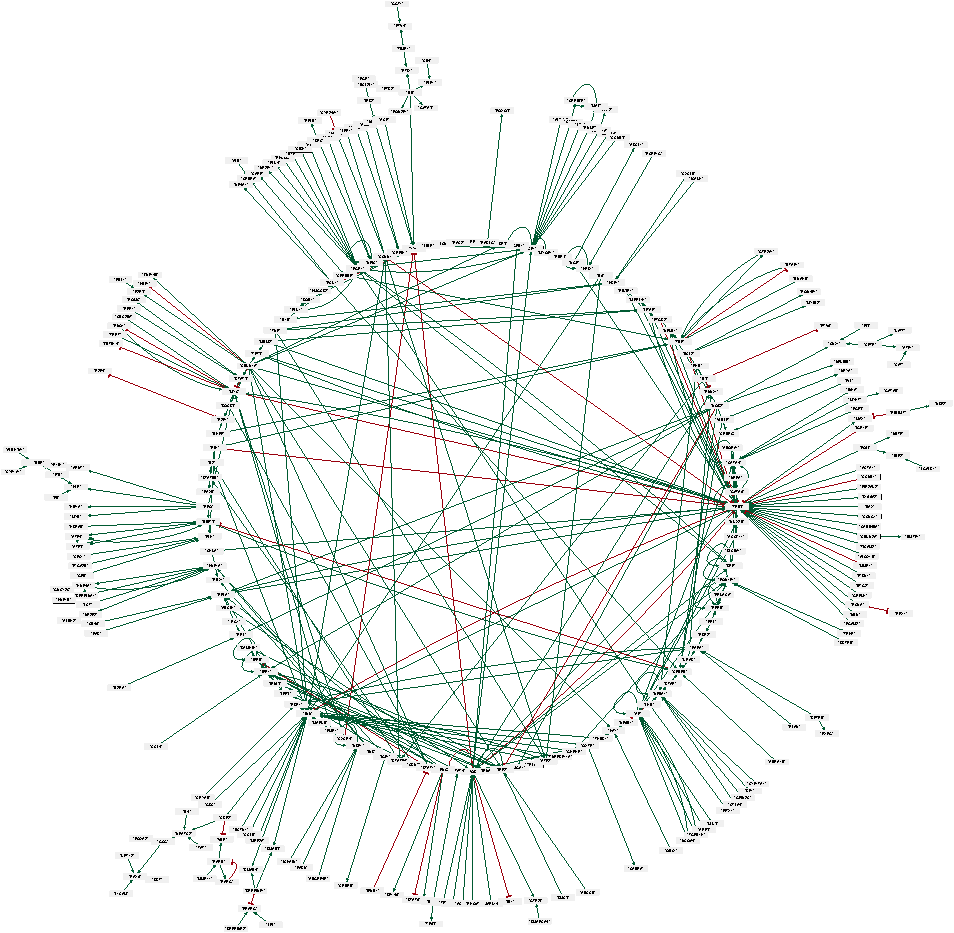
\includegraphics[height=4in]{fig2.2.regulons}
    \caption[Gene regulatory network based on regulon representation of human transcriptional interactions.]{\gls{GRN} based on regulon representation of human transcriptional interactions. CollecTRI-derived regulons were extracted from the decoupleR (v. 2.12.0) package, which provided 43,178 interactions. CollecTRI collection~\cite{RN145} is a comprehensive, curated resource of \gls{TF}s and their target genes, expanding on DoRothEA. This figure illustrates a subset of those 1,000 interactions, with edge color indicating the mode of regulation (green for activation and red for inhibition) using RCy3 (v. 2.26.0) \gls{R} package for visualization.}
    \label{fig:fig2.2.regulons}
\end{figure}

The use of large-scale causal graphs for gene expression data interpretation was first introduced by Pollard \textit{et al.}~\cite{RN131, RN135}. This study aimed to infer the molecular causes of the changes in oxidative phosphorylation gene expression in skeletal muscle from type \gls{DM2} patients. For this purpose, the gene expression data were integrated with a large-scale model created from over 210,000 molecular relationships based on \gls{DM2} literature. 
Computer-aided causal reasoning on these complementary data identified that the observed changes are linked to decreased glucose transport, impaired insulin signaling, and increased risk of post-transplant diabetes~\cite{RN131}.

Given the good results obtained from supplementing the studies with \gls{PKN}, the identification of interactions began to receive more attention. 
The development of high-throughput screening techniques~\cite{RN138} allowed the construction of \gls{PPI}. Which in turn have begun to be deposited in databases that provide molecular interaction data.
Nowadays, there are several public and commercial network and pathway resources, some of them summarized in Table~\ref{tab:interactionsresources}.
Two resources that provide composite public and commercial networks are OmniPath and MetaBase, respectively. OmniPath~\cite{RN91} is a freely available resource of prior knowledge in molecular biology. 
It combines data from over 100 resources and builds five integrated databases with different types of data: Interactions (several molecular interactions organized into sub-networks), Post-Translational Modifications (enzyme-substrate reactions), Complexes (35,000+ protein complexes), Annotations (proteins and complexes annotations, such as the function, localization, tissue, etc.) and Intercell (inter-cellular signaling)~\cite{RN91}. 
The interactions database is a composite signaling network that offers several manually curated subnetworks, encompassing a total of 282,504 unique interactions. 
Each subnetwork has different types of interactions, including post-translational interactions, transcriptional interactions, post-transcriptional interactions, and other interactions involving small molecules. 
The number of interactions per subnetwork is described in Figure~\ref{fig:fig2.3.omnipath}. One of the GRNs that is provided by this database is the CollecTRI-derived regulons~\cite{RN145} (Figure~\ref{fig:fig2.2.regulons}). 
This collection contains high-confidence signed \gls{TF} - target gene interactions compiled from 12 resources, including information inferred from text mining, manual curations, and several publicly available databases.
OmniPath data can be accessed through the OmnipathR \gls{R} package~\cite{RN92}.

\begin{figure}[htbp]
    \centering
    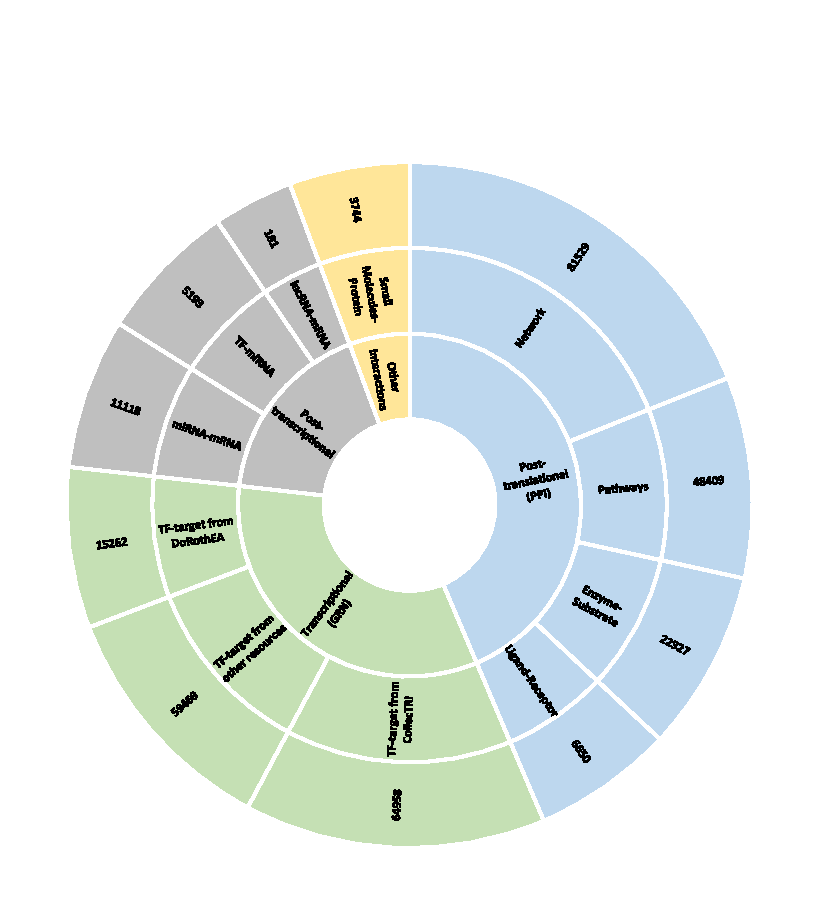
\includegraphics[height=6in]{fig2.3.omnipath}
    \caption[OmniPath molecular interactions database.]{OmniPath molecular interactions database. This figure presents a hierarchical visualization of human molecular interactions curated by OmniPath, which compiles data from diverse resources. The graph displays the numbers of distinct interaction types, including post-translational interactions (\gls{PPI}), transcriptional interactions (\gls{GRN}), post-transcriptional interactions (such as miRNA-\gls{mRNA}, \gls{TF}-miRNA, and lncRNA-\gls{mRNA} interactions), and other interactions involving small molecules (encompassing drug-target, ligand-receptor, enzyme-metabolite, among others).}
    \label{fig:fig2.3.omnipath}
\end{figure}

MetaBase\textsuperscript{TM}~\cite{RN33} is a proprietary, commercial database from Clarivate that offers one of the most comprehensive, manually curated systems biology datasets available. It contains over 4.2 million molecular interactions, including protein-protein, protein-RNA, compound-protein, compound-compound interactions, and transport reactions, with details on directionality, mechanisms, and effects. In addition, MetaBase provides more than 1,500 pathway maps that cover regulatory, disease, metabolic, and toxicity characteristics, alongside over 10,000 disease-related networks and 1,000+ validated networks. Each interaction is assigned a trust score that reflects its reliability, helping users distinguish well-established interactions from those obtained via high-throughput screening. MetaBase can be accessed via metabaseR package in \gls{R}, which simplifies visualization, functional analysis, and network manipulation. Furthermore, the \gls{CBDD} \gls{R} package offers 73 advanced algorithm implementations for analyzing and extracting insights from these networks.

\begin{newpdflayout}{210mm}{297mm}%{420mm}

%\begin{center}
\begin{longtable}{@{} 
  p{0.10\linewidth}@{\hspace{6pt}} 
  p{0.08\linewidth}@{\hspace{6pt}} 
  p{0.69\linewidth}@{\hspace{6pt}} 
  p{0.08\linewidth} 
@{}}
%\begin{longtable}{@{} p{3cm} p{2cm} p{16cm} p{2cm} @{}}
\caption{List of resources that provide prior knowledge networks and pathways.}
\label{tab:interactionsresources} \\ 
\toprule
\textbf{Database} & \textbf{Type of data} & \textbf{Description} & \textbf{Ref.} \\
\midrule
\endfirsthead

\multicolumn{4}{@{}l}{\tablename\ \thetable\ -- \textit{Continued from previous page}}\\
\toprule
\textbf{Database} & \textbf{Type of data} & \textbf{Description} & \textbf{Ref.} \\
\midrule
\endhead

\midrule \multicolumn{4}{r}{\textit{Continued on next page}} \\
\endfoot

\bottomrule
\endlastfoot
BioSNAP & Network & 
  The Biological Stanford Network Analysis Project (\href{http://snap.stanford.edu/}{BioSNAP}) includes multiple biological networks encompassing different entities and relationships, such as a disease-drug association (1,334,088 edges); side effects-drug relationships (4,649,441 edges); tissue-specific protein-protein interactions (70,338 edges), physical protein-protein interactions identified in human (342,353 edges) and many more. BioSNAP also provides a tool, Mambo, for the construction, representation, and analysis of large multimodal networks. &
  ~\cite{RN140} \\
IntAct & Network & 
  \href{https://www.ebi.ac.uk/intact}{IntAct} is a public molecular interaction database with over 1,600,000 interactions, derived from literature curation (23,000+ publications) and user submissions (75,000+ experiments) for multiple species. &
  ~\cite{RN139} \\
KEGG & Pathways &
  Kyoto Encyclopedia of Genes and Genomes (\href{https://www.genome.jp/kegg}{KEGG}) primarily features metabolic pathways but also includes signal transduction and disease-specific data. KEGG Pathway consists of manually curated pathway maps, illustrating molecular interactions, reactions, and networks across various domains, such as metabolism, cellular processes, human diseases, drug development, etc. KEGG covers 578 human pathways, 12,629 drugs (including 2,499 drug groups), and 2,894 human diseases. &
  ~\cite{RN141} \\
MetaBase & Network & 
   MetaBase (MetaBase) provides commercially available manually curated networks, larger (higher number of nodes) and denser (higher number of connections) than other publicly available databases. It contains 4.2 M+ molecular interactions with directionality, mechanism, and effect. Although this is primarily described as a network resource, MetaBase also includes curated pathway maps. It covers human, rat, and mouse genes. metabaseR is a software package that facilitates access to MetaBase content in \gls{R}. &
  ~\cite{RN33} \\
OmniPath & Network & 
  \href{https://omnipathdb.org/}{OmniPath} is a freely accessible resource that integrates molecular biology data into five main databases: Interactions, Post-Translational Modifications, Complexes, Annotations, and Intercellular. The interactions database contains high-confidence data from different sources encompassing 282,504 unique interactions, organized into various subnetworks. Software tools are also provided for R (OmnipathR) and Python (pypath), together with a plug-in for network visualization (OmniPath Cytoscape)~\cite{RN146, RN92}. &
  ~\cite{RN91} \\
Pathway commons  & Pathways &
  \href{https://www.pathwaycommons.org/}{Pathway Commons} is a public repository of pathway and interaction data from 23 databases formatted in the BioPAX standard. It currently includes 6,692 pathways and 3,579,336 interactions from sources like KEGG, IntAct, BioGRID, Reactome, etc. It provides an R package~\cite{RN151}, and the CyPath2 plugin for pathway visualization in Cytoscape. &
  ~\cite{RN142} \\
Reactome & Pathways &
  \href{https://reactome.org/}{Reactome} is a free, open-source, and peer-reviewed pathway database that is manually curated. It includes 2,769 human pathways, 23,911 interactions, 11,574 proteins, and 1,057 drugs, with over 40,000 literature references. The pathways are organized under 29 categories, such as cell-cell communication, signal transduction, etc. Reactome offers a Pathway Browser for visualizing and interacting with the data, as well as an integrated Analysis Tool~\cite{RN150} for pathway identifier mapping, over-representation, and expression analysis. It also provides two R packages, ReactomePA~\cite{RN148} for pathway analysis and ReactomeGSA~\cite{RN149} for Multi-Omics Comparative Pathway Analysis, and the ReactomeFIPlugIn for pathway visualization in Cytoscape. &
  ~\cite{RN143} \\
STRING & Network & 
  \href{https://string-db.org/}{STRING} is a public database that includes known and predicted \gls{PPI}, derived from genomic context predictions, high-throughput lab experiments, co-expression data, automated text mining, and existing databases. STRING currently covers over 59.3 million proteins from 12,535 organisms, providing a comprehensive \gls{PPI} network with confidence scores based on various data sources. &
  ~\cite{RN72} \\
WikiPathways & Pathways &
  \href{https://www.wikipathways.org/}{WikiPathways} iis another open-source curated pathways database. It provides pathways for 27 organisms and includes 959 curated human pathways. The platform supports collaborative annotation and refinement of pathways. It also provides several software tools and workflows in R (rWikiPathways) and Python (pywikipathways), along with Cytoscape and PathVisio plug-ins for pathway visualization, among others~\cite{RN147} &
  ~\cite{RN144} \\
\end{longtable}
%\end{center}

\end{newpdflayout}


Integrating biological knowledge with experimental data is key to understanding how cellular regulation impacts gene expression. Known interaction networks are usually used to predict the results of regulatory events, but they can also be used in the opposite direction, to find upstream regulators that cause expression changes~\cite{RN131}. Computational tools play a crucial role here. They combine high-throughput omics data with established cellular interactions, like \gls{PPI} and signaling pathways, to give a broader context. While network data show the complete interactome of molecular interactions, pathway data arrange these interactions into cascades. Each of these data sources forms prior knowledge. When combined with experimental results helps to create mechanistic hypotheses about, for instance, how a perturbation works in a system. This integration of experimental and interaction data sets the stage for some of the computational methods covered in the next chapter. These methods aim to uncover the mechanisms that cause an observed transcriptomic change.

\section{Computational methods for MoA inference} % (fold)
\label{sec:ComputationalmethodsforMoAinference}

Due to technological advances, large-scale transcriptomic datasets can now be generated affordably for many perturbations. 
However, extracting biological insights from this data can be complicated, requiring dedicated computational tools for the analysis. 
These methods include \textit{in silico} experiments that combine experimental data with prior knowledge. 
They fall into three main categories: topology-based, similarity, and enrichment methods~\cite{RN57, RN56}. 
Choosing the appropriate tool depends on several factors, including the type of input data, runtime, computational complexity, and the specific scientific questions being addressed, along with the inherent strengths and limitations of each method~\cite{RN38}. 
For example, in Hill \textit{et al.}'s study,~\cite{RN37} three types of topology-based algorithms were employed. 
Node prioritization algorithms rank the nodes in the network based on the distance from start nodes and the connection between them; causal regulation algorithms infer and rank upstream nodes in the network by combining the direction of edges, and subnetwork identification algorithms extract regions of the input network that are enriched for perturbed nodes. 
These approaches help generating mechanistic hypotheses about the cellular targets and pathways affected by a perturbagen, more efficiently and accurately~\cite{RN100}. 

\subsection{Connectivity-based tools for comparative analysis} % (fold)
\label{sub:connectivity-basedmethods}

Similarity-based approaches for \gls{CMap} focus on matching gene expression signatures from query to reference signatures. 
The approach emerged from the need to connect changes caused by perturbagens, with those observed in diseased or other biological states.
As stated by Lamb \textit{et al.}~\cite{RN34} the resource was named \gls{CMap}, due to its potential to connect drugs, genes, and diseases, with the foundational idea that if a compound induces a transcriptional signature similar to a known gene expression pattern, it likely shares the same \gls{MoA} or therapeutic effect. 
The two main components of this approach are: a query signature, a ranked list of genes up- or downregulated in a condition of interest and a reference database.  
Using a pattern-matching algorithm, the query signature is systematically compared against a reference database of perturbation-induced expression profiles~\cite{RN155}. 
The seminal study that proposed the first connectivity-based approach also introduced the first \gls{CMap} database, described in section~\ref{sec:Transcriptomicdata}. 
As a strategy to score the similarity between data, the authors employed a nonparametric, rank-based \gls{KS} test~\cite{RN34, RN79}. 
This approach has been adapted and extended by several methods, including those based on weighted \gls{KS} statistics, such as the variations of the \gls{GSEA}, and alternative metrics such as the \gls{XSum} score and signed rank-based methods like the ZhangScore~\cite{RN79}. 

For each reference profile, the algorithm evaluates whether query upregulated genes cluster near the top of the ranked list and downregulated genes near the bottom, indicating a positive connection, or a negative connection. 
This yields a connectivity score between 1 (strong concordance) and -1 (strong anticorrelation), with scores near zero indicating no significant association~\cite{RN34}. 
In this way, these methods not only generate the direction of correlation, but also provide information on the strength of the link. 
The similarity scores can be directly linked to biological interpretations. 
A high positive score may indicate that a compound could enhance a biological condition, while a high negative score suggests a potential inhibitory effect~\cite{RN102}. 

\gls{CMap} has become a powerful tool for \gls{DR} and mechanistic studies because it leverages large-scale gene expression data, to connect drugs, diseases, and gene perturbations. 
By comparing a query signature with a database of perturbagen signatures, candidate drugs that may reverse or have similar transcriptional changes patterns can be identified~\cite{RN102}. The \gls{CMap} concept not only facilitated the creation of several drug-induced molecular perturbation signature databases~\cite{RN84}, but also supported studies applying similarity-based algorithms in \gls{DR} and \gls{MoA} elucidation~\cite{RN86}. 
% Consequently, this resulted in prediction and experimental validation of novel applications for existing drugs.

\subsection{Enrichment-based tools for downstream analysis} % (fold)
\label{sub:enrichmentbasedtools}

As the number of gene expression studies increases, it becomes harder to extract relevant information. Pathway analysis helps to frame large changes in gene expression that, if isolated, lack biological context. These methods convert gene lists into a meaningful and interpretable biological process, by linking expression data to specific biological pathways.

Biological pathways are identified by characterizing the cascade of interactions occurring in the system in response to a given perturbation. These interactions can be observed in transcriptomic data and translated into significantly enriched pathways, to capture how changes in gene expression are preferentially affecting some pathways more than others. However, pathway analysis does not trace the causal paths leading to observed gene expression. One commonly used method to detect these relevant pathways is \gls{GSEA}. The input for \gls{GSEA} is a ranked list of genes, based on metrics like fold-change and a predefined gene set. The algorithm then checks if each gene from the gene sets cluster at the top or bottom of the ranked list, and calculates an \gls{ES}. The statistical significance is evaluated using a \gls{KS} test~\cite{RN152}. 
Since it is a rank-based approach, there is no need to use thresholds (for example, for fold-change), a full gene expression profile can be used, not only \gls{DEGs}. This reduces bias and increases sensitivity to pathways where individual gene changes are small but consistent. However, this thoroughness comes with a high computational cost.

\gls{ORA}, on the other hand, is a simpler and faster method for pathway enrichment. It is ideal for large-scale screening and initial data exploration. This analysis uses a hypergeometric test or Fisher's exact test, a background gene set and list of genes of interest, meeting a specific fold-change or statistical threshold (such as \gls{DEGs}). The statistical test compares the overlap between the input gene list and each pathway for each gene in the list. Since \gls{ORA} only needs a non-ranked gene list, it can be more straightforward than \gls{GSEA}. However, by relying on a cutoff for the input list the pathway detection is affected by a certain degree of subjectivity. 
Additionally, \gls{ORA} does not consider the magnitude or direction of gene expression changes and, by assuming independence among genes and pathways, it may overlook complex interactions. 

Overall, enrichment-based methods help provide a broader and better view of biological processes affected downstream of transcription. However, they lack the context of mechanisms behind observed changes.
One way to understand the how and why those changes are observed in the gene expression data is through topology-based algorithms.
These algorithms can combine transcriptomic data with network information to predict drug or disease targets.


\subsection{Topology-based methods for upstream analysis} % (fold)
\label{sub:topologybasedmethodsforupstreamanalysis}

While pathway enrichment methods compare gene expression data with the respective encoded proteins and the signaling pathways, on the other hand, topology-based methods treat a gene expression pattern as the result of a specific perturbation. Several algorithms fall into the category of topology-based methods, as they take advantage of a topology network as prior knowledge. A subset of them is categorized as causal reasoning algorithms. Causal reasoning can be described as the process of looking at what happened, the effects, and trying to infer the upstream causes. In this context, change in a process in response to specific stimulus is considered as a proxy for causality, in line with the following axiom A causes B if a change in A leads to a difference in B, assuming everything else stays the same.~\cite{RN157}. This thinking has deep philosophical roots, and, in systems biology, it has a more testable and specific meaning. In early medical applications of causal reasoning, A represented the treatment, and B was the outcome. 

In \gls{DD} studies, this concept can be applied by overlaying high-throughput measurements, such as gene expression data, onto a network. 
The algorithm itself is a sophisticated causal node prioritization tool that makes predictions based on network topology. 
It requires direct interactions, meaning directed cause-effect relationships, connecting each pair of biological entities. 
Additionally, it uses edge effects, to know (at least for some edges) whether it represents activation or inhibition. 
For \gls{DEGs}, it doesn't necessarily require the exact fold-change values; instead, it is sufficient to specify which genes are up- and down-regulated. 
At its core, a causal reasoning algorithm works backward. It starts with a node in the network and follows it downstream for a few steps, predicting what would happen if this node were activated (or inhibited) in the biological system of interest. 
For example, by analyzing the network structure, it can determine if the activation of a specific regulatory protein will also activate a certain TF, directly affecting the expression of target genes in a positive or negative way (respectively by activating or repressing gene expression). 
The algorithm makes these predictions and then compares them with what is observed in the data. 
This helps identify which upstream regulators best explain the downstream changes that are seen~\cite{RN32}. However, not every edge in a prior network is active during a specific experiment, and not all predicted downstream effects occur. 
This is the reason why statistical scoring is crucial. In causal-network inference, all evaluation methods compare each regulator predicted downstream effects against the observed gene expression changes, but the exact scoring metric depends on the type of network used~\cite{RN81}. 
The simplest approach merely counts how many predictions are correct and incorrect. A more refined \gls{ES} uses Fisher's exact test to evaluate whether the targets of a regulator are enriched among the differentially expressed genes while ignoring whether each edge is activated or inhibited. 
To capture that extra layer of information, the \gls{QS} computes a z-score to quantify how well the predicted up/down directions match the observed up/down changes in the data~\cite{RN156}. 
Early work by Pollard \textit{et al.}~\cite{RN135} combined the two methods, computing an overlap and concordance p-values for regulators in type-2 diabetes expression data~\cite{RN156}.  
However, Fisher's test cannot leverage signed edges even when those signs are known.
To address this, Chindelevitch \textit{et al.}~\cite{RN73, RN131} developed a \gls{TS} method that models the signed network and observations as a dot-product distribution, allowing exact p-values for both the activation and inhibition hypotheses of each regulator. 
This scoring method requires a fully annotated causal graph, i.e., every edge must have a known direction and effect information. 
More recently, Fakhry \textit{et al.}~\cite{RN158} introduced a \gls{QS} method that extends TS to networks containing both signed and unsigned interactions, preserving directional inference wherever possible while still accommodating unannotated edges~\cite{RN81}. 
Early methods used simpler calculations, while newer methods used more precise statistical tests to ensure accuracy. However, simpler z-score and enrichment-based methods are still popular because they are faster to compute and easier to use and understand. 
Causal reasoning algorithms are widely used but have many nuances depending on the network's structure and how far one can trace from regulators to downstream genes.
Improving its accuracy in predicting regulators is a key focus. Also, they are complex and computationally demanding, especially with the increase in input data.

There are evidences that topology-based methods may be more useful in \gls{DD} than pathway enrichment methods.
Topology-based causal reasoning takes advantage of directed and signed \gls{Molecular network}s to infer the most plausible upstream regulators from transcriptomic endpoints.
By inferring key signaling nodes whose activity can directly explain the changes observed in the experimental data, these methods pinpoint candidate drug targets and generate mechanistic hypotheses for further validation. 
On the other hand, pathway enrichment methods only infer which biological processes are affected by changes in gene expression.
These methods do not consider that after transcription, events such as translation and post-translational modifications will also affect protein activity~\cite{RN53}.

\section{Benchmarking of computational methods for MoA inference} % (fold)
\label{sec:benchmarkingofcomputationalmethodsforMoAinference}

The use of computational methods to elucidate \gls{MoA} is becoming increasingly indispensable for integrating and interpreting multidimensional biological data. 
Given the plethora of existing computational tools, choosing the appropriate data and methods to answer specific scientific questions can be challenging.
When a new tool is developed and published, it is usually benchmarked against popular existing methods.
Without a deep expertise in the area, distinguishing the benefits of a novel tools can be difficult. 

A comprehensive benchmarking study is crucial for evaluating available methods in a standardized way, providing sufficient information to accurately choose the best tools and data for a given study~\cite{RN108}.
A key component of a benchmarking study is the use of gold-standard datasets, against which results are compared.
By this process, often formalized via well-defined good practises, it is possible to evaluate performance metrics and statistical analyses and to compare different algorithms on specific types of data. 

Benchmarking studies can be carried out by the authors that implemented the tool, independent groups, or as organized challenges, such as those by the Dialogue on Reverse Engineering Assessment and Methods (DREAM) Consortium~\cite{RN109}.
If the evaluation is performed by the authors, the aim is usually to demonstrate the advantages and performance improvements over other techniques.
In other contexts, it is important to define the benchmark's scope and purpose.
The selection of the methods should reflect the relevance of the study's objective and include publicly available implementations to ensure accessibility.
Parameter optimization can significantly affect a tool's behavior, including runtime, yet finding the optimal values is not always straightforward.
Thus, balancing default settings with computational efficiency is important.
Regarding datasets, in \gls{MoA} studies, it is crucial to include diverse data sources and generation methods, to ensure representativity and a credible assessment of performance.
For instance, transcriptomic data should ideally include both bulk \gls{RNA-seq} and \gls{scRNA-seq} data to broaden the options and use two widely used types of data.
Since there are no perfect, fully curated datasets, it is necessary to ensure quality, to avoid biasing the results and performance of the tools~\cite{RN109}.
The same applies to the gold standard datasets, which serve as the ground truth, and they represent the essence of a benchmarking study.

Other similar studies arise from an effort to contextualize gene expression data with several computational algorithms.
Hosseini-Gerami \textit{et al.}~\cite{RN53} evaluated the performance of different causal reasoning algorithms to recover direct targets of small molecules and associated signaling pathways using gene expression data.
The study compared four causal reasoning algorithms against networks from two diverse sources and transcriptomic data from one database.
Hill \textit{et al.}~\cite{RN37} conducted a study that provided a more comprehensive framework, by analyzing a diverse range of algorithms, networks, and datasets to assess how well network-based algorithms prioritize and connect gene lists derived from transcriptomic data.
This study integrated 17 algorithms, categorized into three main groups: (1) Node prioritization algorithms, which rank network nodes based on connectivity, (2) Causal regulator algorithms, which identify upstream regulators of gene expression changes, and (3) Subnetwork identification algorithms, which extract subnetworks linking input genes.
The algorithms were applied to three \gls{PPI} networks, each with different structures and levels of curation, using hundreds of datasets from four sources to cover scenarios where certain data types might be unavailable.
The first network combined data from various sources, resulting in a mix of signed/unsigned and directed/undirected interactions.
The second network included only signed, directed, and high-confidence interactions, while the third was a large-scale, undirected \gls{PPI} network.
This study exemplifies good practices when comparatively analyzing different algorithms and integrating different resources, although it does not explore the algorithms' parameter landscape (considered beyond the scope of the work).

Typically, a benchmarking analysis ranks the algorithms in terms of the most appropriate use for distinct applications, and so the choice of algorithm(s) may depend on the specific use case~\cite{RN37}.
By providing a robust assessment of the capabilities of existing algorithms, these studies provide guidelines for researchers to choose the most appropriate tool for the scientific question of interest~\cite{RN108}.

